\documentclass[11pt]{article}
\usepackage{amsmath, amssymb, array}
\pagestyle{plain}

\textwidth=6.5in
\hoffset-1in
\textheight=9in
\voffset-1in

\usepackage{enumitem}
\usepackage{pgfplots}
\usepackage{graphicx}
\usepackage{lipsum}
\usepackage{stfloats}
\usepackage{multicol}
\usepackage{minipage-marginpar}
\usepackage{tikz}
\setlength{\columnsep}{1cm}
\usepackage{pinlabel} % for pin labels on figure


\newcommand{\abs}[1]{\left| #1 \right|}


\begin{document}


\noindent MATH 1113   \quad\quad\quad\quad\quad Worksheet \quad\quad\quad\quad\quad\   Name \underline{\phantom{alphabetsoupismyveryveryfavorite}}\\ 
\noindent Section 2.2 \\




\noindent \textbf{Instructions:}  Work together in groups of  3 or 4 to complete the following problems.\\

\begin{enumerate}



\item Circle the polynomial functions.
$$g(x)=-3x^5+\sqrt{2}x+\frac{1}{2}x \quad \quad \quad \quad h(x)=-3x^2+2\sqrt{x}+\frac{2}{x}$$ 
\vfill
$$k(x)=\sin(x+5)-2 \quad \quad \quad \quad j(x)=3(x-1)^3(x+2)^2(x-5) \quad \quad \quad \quad r(x)=7$$
\vfill
\item Determine the end behavior of the graph of the following function.
\begin{enumerate}
\item $f(x)=-3x^4-5x^2+2x-6$
\vfill
\vfill
\item $g(x)=-\frac{1}{2}x^6+8x^4-x^3+9$
\vfill
\vfill
\item $h(x)=-5x^4(2-x)^3(2x+5)$
\vfill
\vfill
\end{enumerate}

\newpage


\item Find the zeros of the function and state the multiplicities.

\begin{enumerate}

\item $f(x)=x^3+2x^2-25x-50$
\vfill
\item $g(x)=x^3+5x^2-x-5$
\vfill



\item $h(x)=-6x^3-9x^2+60x$

\vfill

\newpage
\item $p(x)=-3x(x+3)^3(x+4)$

\vfill
\vfill

\item $n(x)=x^6-7x^4$
\vfill
\vfill
\end{enumerate}

\item Determine whether the intermediate value theorem guarantees that the function \\$f(x)=2x^3-7x^2-14x+30$ has a zero on the given interval.
\begin{enumerate}
\item $[1,2]$
\vfill
\item $[2,3]$
\vfill
\item $[3,4]$
\vfill
\end{enumerate}

\newpage

\item Determine if the graph can represent a polynomial function.  If so, assume that the end behavior and all turning points are represented on the graph.


\begin{itemize}
\item Determine the minimum degree of the polynomial.
\item Determine whether the leading coefficient is positive or negative based on the end behavior.
\item  Determine whether the degree of the polynomial is even or odd.
\item Approximate the real zeros of the function and determine if their multiplicities are even or odd.\\
\end{itemize}


\begin{multicols}{2}

\begin{enumerate}

\item \ 

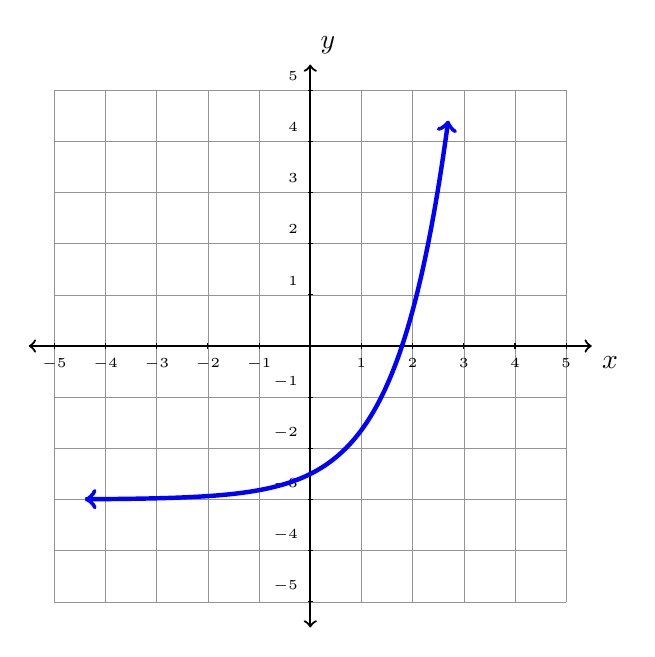
\begin{tikzpicture}[y=.65cm, x=.65cm,font=\sffamily,
	mydot/.style={
    circle,
    fill=white,
    draw,
    outer sep=0pt,
    inner sep=1.5pt
  }]
    %% Add a grid
    \draw[step = 1, gray, very thin,opacity=0.85] (-5, -5) grid (5, 5);
 	%% Draw the axes
	\draw[thick,<->] (-5.5,0) -- coordinate (x axis mid) (5.5,0) node[anchor = north west] {$x$};
    \draw[thick,<->] (0,-5.5) -- coordinate (y axis mid) (0,5.5) node[anchor = south west] {$y$};
    %% Label the y axis
    \foreach \y in {-5,...,-1,1,2,...,5} {
      \draw (1pt, \y) -- (-1pt, \y) node[anchor = south east] {\tiny $\y$};
    }
    %% Label the x axis
    \foreach \x in {-5,...,-1,1,2,...,5} {
      \draw (\x,1pt) -- (\x,-1pt) node[anchor = north] {\tiny $\x$};
    }
    %% Draw the function.
    \begin{scope}
%         \draw[very thick,blue] (-3,2) -- (1,1);
%         \draw[very thick,blue] (3.05,1.05) -- (4,3);
%         \draw[very thick,blue] (1.1,4) -- (3,4);
    %semi-circle
         %\draw[very thick, blue] (1,1) arc [radius=1, start angle=180, end angle= 5];
     %parabola
         %\draw[ultra thick, blue, domain=-5:0] plot (\x, {(-0.2)*(\x-5)*(\x+5)});
         \draw[ultra thick, blue, <->, domain=-4.4:2.7] plot[samples=1000] (\x, {.5*e^\x-3)});             %dots
%         \fill[blue] (-3, 2) circle[radius=0.5ex];
%         \fill[blue] (1,1) circle[radius=0.5ex];
%         \fill[blue] (4,3) circle[radius=0.5ex];
%         \draw[very thick, blue] (3,1) circle[radius=0.5ex];
%         \fill[blue] (3,4) circle[radius=0.5ex];
%         \draw[very thick, blue] (1,4) circle[radius=0.5ex];


    \end{scope}

    %%\node[above=0.1cm] at (-2,2 )   {\nextXValue};

\end{tikzpicture}

\item \ 


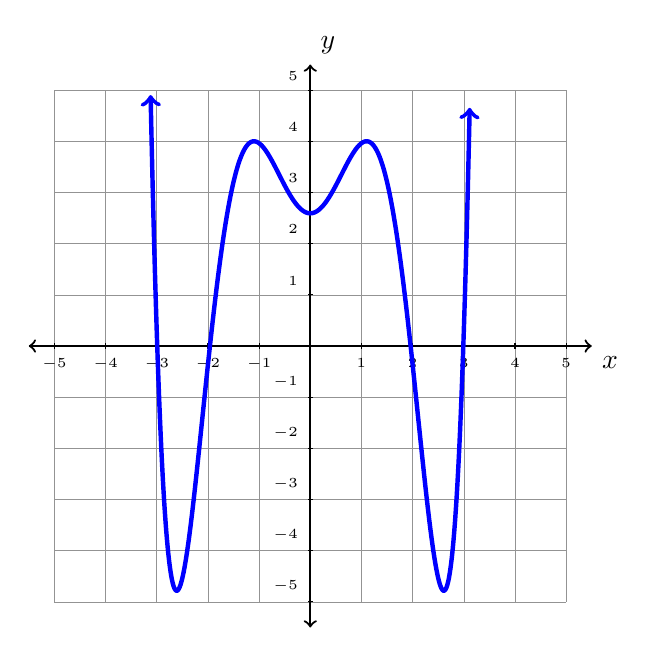
\begin{tikzpicture}[y=.65cm, x=.65cm,font=\sffamily,
	mydot/.style={
    circle,
    fill=white,
    draw,
    outer sep=0pt,
    inner sep=1.5pt
  }]
    %% Add a grid
    \draw[step = 1, gray, very thin,opacity=0.85] (-5, -5) grid (5, 5);
 	%% Draw the axes
	\draw[thick,<->] (-5.5,0) -- coordinate (x axis mid) (5.5,0) node[anchor = north west] {$x$};
    \draw[thick,<->] (0,-5.5) -- coordinate (y axis mid) (0,5.5) node[anchor = south west] {$y$};
    %% Label the y axis
    \foreach \y in {-5,...,-1,1,2,...,5} {
      \draw (1pt, \y) -- (-1pt, \y) node[anchor = south east] {\tiny $\y$};
    }
    %% Label the x axis
    \foreach \x in {-5,...,-1,1,2,...,5} {
      \draw (\x,1pt) -- (\x,-1pt) node[anchor = north] {\tiny $\x$};
    }
    %% Draw the function.
    \begin{scope}
%         \draw[very thick,blue] (-3,2) -- (1,1);
%         \draw[very thick,blue] (3.05,1.05) -- (4,3);
%         \draw[very thick,blue] (1.1,4) -- (3,4);
    %semi-circle
         %\draw[very thick, blue] (1,1) arc [radius=1, start angle=180, end angle= 5];
     %parabola
         %\draw[ultra thick, blue, domain=-5:0] plot (\x, {(-0.2)*(\x-5)*(\x+5)});
         \draw[ultra thick, blue, <->, domain=-3.12:3.12] plot[samples=1000] (\x, {.1*(\x-1.1)^2*(\x+1.1)^2*(\x-3.1)*(\x+3.1)+4});
           %dots
%         \fill[blue] (-3, 2) circle[radius=0.5ex];
%         \fill[blue] (1,1) circle[radius=0.5ex];
%         \fill[blue] (4,3) circle[radius=0.5ex];
%         \draw[very thick, blue] (3,1) circle[radius=0.5ex];
%         \fill[blue] (3,4) circle[radius=0.5ex];
%         \draw[very thick, blue] (1,4) circle[radius=0.5ex];


    \end{scope}

    %%\node[above=0.1cm] at (-2,2 )   {\nextXValue};

\end{tikzpicture}

\columnbreak

\item \ 

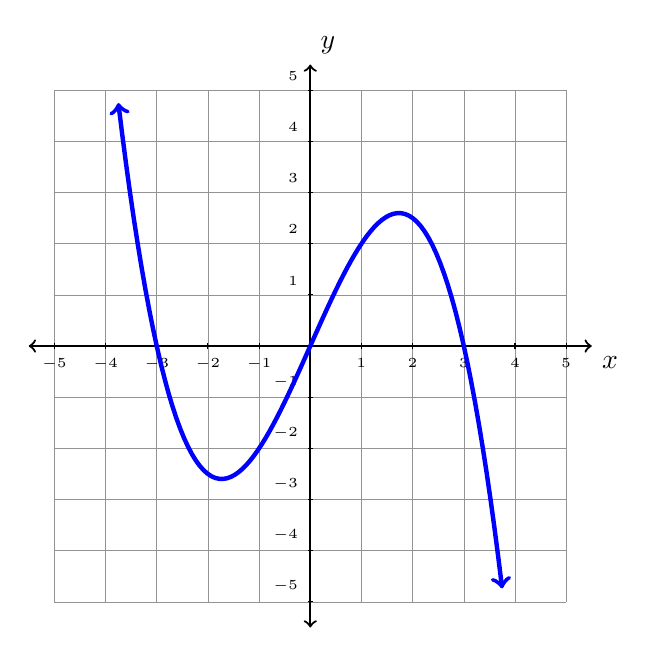
\begin{tikzpicture}[y=.65cm, x=.65cm,font=\sffamily,
	mydot/.style={
    circle,
    fill=white,
    draw,
    outer sep=0pt,
    inner sep=1.5pt
  }]
    %% Add a grid
    \draw[step = 1, gray, very thin,opacity=0.85] (-5, -5) grid (5, 5);
 	%% Draw the axes
	\draw[thick,<->] (-5.5,0) -- coordinate (x axis mid) (5.5,0) node[anchor = north west] {$x$};
    \draw[thick,<->] (0,-5.5) -- coordinate (y axis mid) (0,5.5) node[anchor = south west] {$y$};
    %% Label the y axis
    \foreach \y in {-5,...,-1,1,2,...,5} {
      \draw (1pt, \y) -- (-1pt, \y) node[anchor = south east] {\tiny $\y$};
    }
    %% Label the x axis
    \foreach \x in {-5,...,-1,1,2,...,5} {
      \draw (\x,1pt) -- (\x,-1pt) node[anchor = north] {\tiny $\x$};
    }
    %% Draw the function.
    \begin{scope}
%         \draw[very thick,blue] (-3,2) -- (1,1);
%         \draw[very thick,blue] (3.05,1.05) -- (4,3);
%         \draw[very thick,blue] (1.1,4) -- (3,4);
    %semi-circle
         %\draw[very thick, blue] (1,1) arc [radius=1, start angle=180, end angle= 5];
     %parabola
         %\draw[ultra thick, blue, domain=-5:0] plot (\x, {(-0.2)*(\x-5)*(\x+5)});
         \draw[ultra thick, blue, <->, domain=-3.75:3.75] plot[samples=100] (\x, {(-.25)*(\x-3)*(\x)*(\x+3)});
           %dots
%         \fill[blue] (-3, 2) circle[radius=0.5ex];
%         \fill[blue] (1,1) circle[radius=0.5ex];
%         \fill[blue] (4,3) circle[radius=0.5ex];
%         \draw[very thick, blue] (3,1) circle[radius=0.5ex];
%         \fill[blue] (3,4) circle[radius=0.5ex];
%         \draw[very thick, blue] (1,4) circle[radius=0.5ex];


    \end{scope}

    %%\node[above=0.1cm] at (-2,2 )   {\nextXValue};

\end{tikzpicture}

\item \ 

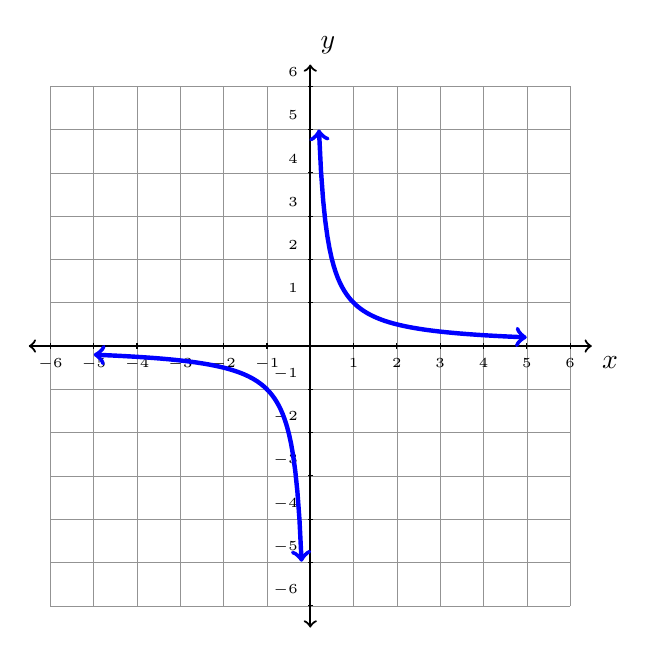
\begin{tikzpicture}[y=.55cm, x=.55cm,font=\sffamily,
	mydot/.style={
    circle,
    fill=white,
    draw,
    outer sep=0pt,
    inner sep=1.5pt
  }]
    %% Add a grid
    \draw[step = 1, gray, very thin,opacity=0.85] (-6, -6) grid (6, 6);
 	%% Draw the axes
	\draw[thick,<->] (-6.5,0) -- coordinate (x axis mid) (6.5,0) node[anchor = north west] {$x$};
    \draw[thick,<->] (0,-6.5) -- coordinate (y axis mid) (0,6.5) node[anchor = south west] {$y$};
    %% Label the y axis
    \foreach \y in {-6,...,-1,1,2,...,6} {
      \draw (1pt, \y) -- (-1pt, \y) node[anchor = south east] {\tiny $\y$};
    }
    %% Label the x axis
    \foreach \x in {-6,...,-1,1,2,...,6} {
      \draw (\x,1pt) -- (\x,-1pt) node[anchor = north] {\tiny $\x$};
    }
    %% Draw the function.
    \begin{scope}
%         \draw[very thick,blue] (-3,2) -- (1,1);
%         \draw[very thick,blue] (3.05,1.05) -- (4,3);
%         \draw[very thick,blue] (1.1,4) -- (3,4);
    %semi-circle
         %\draw[very thick, blue] (1,1) arc [radius=1, start angle=180, end angle= 5];
     %parabola
         %\draw[ultra thick, blue, domain=-5:0] plot (\x, {(-0.2)*(\x-5)*(\x+5)});
         \draw[ultra thick, blue, <->, domain=-5:-.2] plot[samples=100] (\x, {1/\x});
         \draw[ultra thick, blue, <->, domain=.2:5] plot[samples=100] (\x, {1/\x});
     
           %dots
%         \fill[blue] (-3, 2) circle[radius=0.5ex];
%         \fill[blue] (1,1) circle[radius=0.5ex];
%         \fill[blue] (4,3) circle[radius=0.5ex];
%         \draw[very thick, blue] (3,1) circle[radius=0.5ex];
%         \fill[blue] (3,4) circle[radius=0.5ex];
%         \draw[very thick, blue] (1,4) circle[radius=0.5ex];


    \end{scope}

    %%\node[above=0.1cm] at (-2,2 )   {\nextXValue};

\end{tikzpicture}


\end{enumerate}



\end{multicols}





\newpage
\begin{center}
\includegraphics[scale=.6]{heart}
\end{center}
\item The graph shows the heart rate of a person watching a short film, where $x$ represents time in minutes, and $y$ represents heart rate in beats per minute.  Answer the following questions.
\begin{enumerate}
\item For which time periods were the person's heart rate increasing?
\vfill
\item For which time periods were the person's heart rate decreasing?
\vfill
\item How many turning points occurred for the person't heart rate during the 15 minute film?
\vfill
\item Suppose that a polynomial function is used to model the data displayed by the graph.  What is the degree of the polynomial function of best fit?
\vfill
\item For the model in part $(d)$, should the leading coefficient of the polynomial function be positive or negative?  Why?
\vfill
\item Use the graph to estimate the person's maximum heart rate during the 15 minute film.  After how many minutes did this maximum heart rate occur?
\vfill
\item Use the graph to estimate the person's minimum heart rate during the 15 minute film.  After how many minutes did this minimum heart rate occur?
\vfill

\end{enumerate}
\newpage
\item Sketch the graph of $f(x)=x^5-2x^4$.


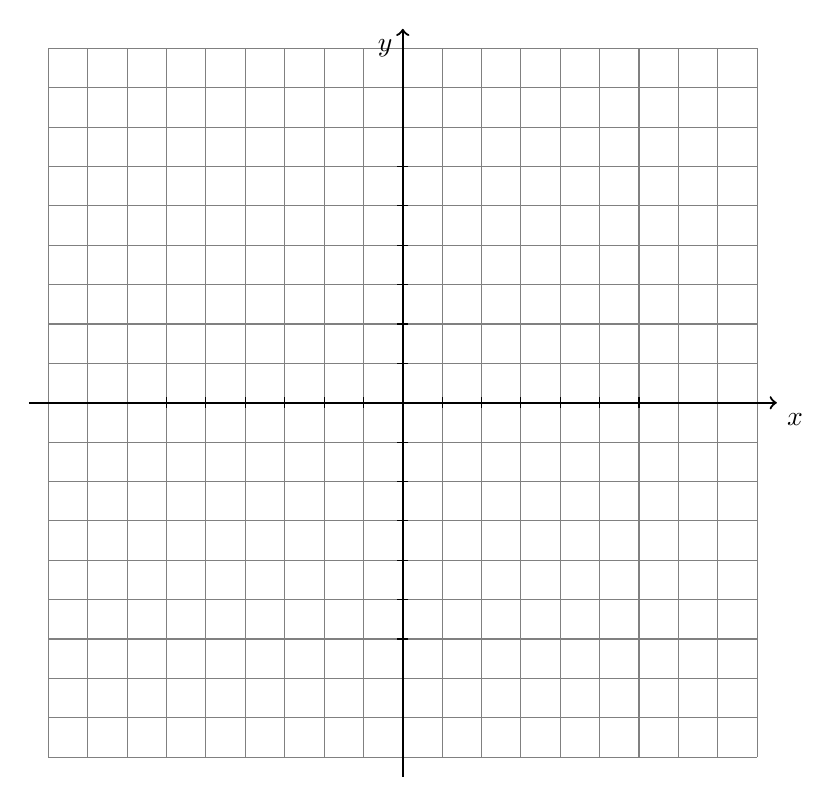
\begin{tikzpicture}[y=.5cm, x=0.5cm,font=\sffamily]
    %% ticks
    \draw[step = 1, gray] (-9,-9) grid (9,9);
    %% axis
    \draw[thick,->] (-9.5,0) -- coordinate (x axis mid) (9.5,0) node[anchor = north west] {$x$};
    \draw[thick,->] (0,-9.5) -- coordinate (y axis mid) (0,9.5) node[anchor = north east] {$y$};
    \foreach \y in {-6,-5,...,-1,1,2,...,6} {
      \draw (2pt, \y) -- (-2pt, \y);
    }
    \foreach \x in {-6,-5,...,-1,1,2,...,6} {
      \draw (\x,2pt) -- (\x,-2pt);
    }

  \end{tikzpicture}


\end{enumerate}

\end{document}